




\maketitle {}

\section{Introduction}
Lecture 4 was covered mostly hands on material paired with a little bit of lectures. He will go into detail about R, and certain programs within R. You might ask why even use R? According to master Hofman "R isn't the best programming language out there, but it happens to be great for data analysis... and when you first start to learn it, the first couple weeks will be you banging your head against the wall, only then you'll be able to show your skills." R provides the user an extremely fast exploratory data analysis, that easily generates high-quality data visualizations, and also fits pretty much any statically model you can think off, as you can see in figure one. The first half of class will talk about how data is manipulated in R, and then the second half we will discuss data visualisation.
\begin{figure}[h!]
  \caption{ Shows varity of statisical models in R (Lecture 4 slides)}
  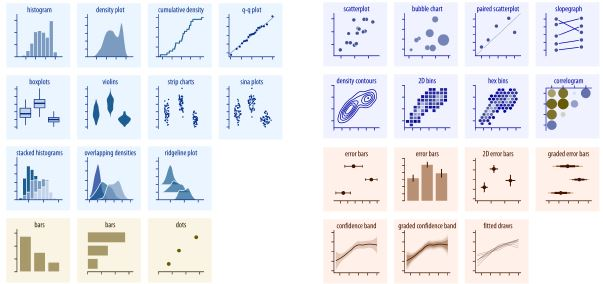
\includegraphics[width=\textwidth]{figures/MSDimage1}
\end{figure}

\section{First Half of Class - Data Manipulations}
\subsection{Lecture Slides - Lecture 3 Slides}
During this subsection we will talk about the basic components of R. in R, there are basic types of variables integer, double (for numbers), character(for strings), factor (for categorical variables). Can also do containers; vector (for multiple values of the same type i.e. array), list (for multiple values of different types i.e. dictionary), and, what we will mostly use, data.frame (for tables of rectangular data of mixed types i.e. a matrix). 

Installing tidyverse is a must!! Every part of this class will use the package, and all of its components, so download it. Tidyverse is a unified interface that is a collection of packages that works together to make data analysis easier such as dply (for split/apply/ and combine type counting), ggplot (for those bomb graphs we will make, like in Figure 1), tidyr for reshaping data, readr for reading and writing files, and many more. However the core philosophy is that your data should be in a "tidy" table with : one variable per column, one observation per row, one measured value per cell, as seen in Figure 2. \begin{figure}[h!]
  \caption{ Tidy Data (Lecture 3 slides)}
  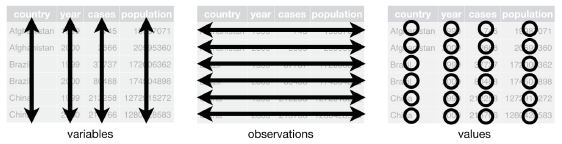
\includegraphics[width=\textwidth]{figures/MSDimage2}
\end{figure} One imporant function function in R is dplyr. For dplyr, it is mostly for a grammar of data manipulation. dplyr implements the split/apply/combine framework discussed in the last lecture (see slide for more detail). The filter function, can separate you data into nice column space. Notice that in the filter function the column names are in scope. We can also use the arrange function to then arrange your data in a certain order, you can also yous the assignment operator <- in R. The Select function is for certain columns of your data that you want, it can also rename your data if so chooses. The mutate function, literally mutates your data such that you can change the data to something you want (EX. change trip time in hours to trip time to minutes). The summarize function takes the data and makes it a one row summary of your input into your summarize function (such as mean and std). The Group-by function takes the data a groups it to the parameters you specify (trips-by-gender <- group-by(trips, gender), note that it is recommended to always ungroup a the end. Note that the group-by and summarize functions can be used together, such that you can summarize the grouped data by more parameters giving a more than one row product. Tee pipe operator takes your data, trips and is the more fluent way to do the summarize and group-by function. 

For untidy data, data is...well isn't pretty and needs to be restructure we follow these commands. The function gather takes your data from "wide to long", it takes the multiple columns of data and combines them such that they're in one column, which will help with when you want to count (hint hint this is on the homework). You can also use the gather function and then mutate functions to give us additional data to how we want it (see slide 22/25). Notice that you can also undo the data set, the spread function will take your from long to wide. They are not inverses ("pretty darn close to being the inverse, but it is not in industry" - Hoffman), as the order is not guaranteed as it will failed if we do not have a complete data set, if we mutate our data  (slide 24/25). All of this is in the Hadley book, there is also a tidyverse stlye guide website that has a walk through for functions and is recommended to look at. 

\subsection{In R Studio - Lecture 3 - Intro to R}
Notice the R is nice enough to use your mouse in. There is a four panel view: top left is the Script, the bottom left is the console and your terminal, bottom right is the plot view/packages installer, and top right is the environments for your data. In class we talked about vectors, factors, how to make lists, and most importantly data frames. We also went into have we used the functions mentioned in the lecture slides above and what they did for an example data frame. For exact examples and more thorough investigation please visit Professors Hofman's Github. 
DISCLAIMER: I am new to R, and it is highly highly recommended you look at lecture 3's Intro to R. 

\section{Second Half of Class}
\subsection{Lecture 4 Slides: Visualizing Data}
Data Visualization is a key aspect in the modern world, as it shows findings to the public.  For example in Figure 3, Ansombe's quartet is a good representation of why choosing visualization is extremely important as summary data can be misleading \begin{figure}[h!]
  \caption{ Anscombe's (Lecture 4 slides)}
  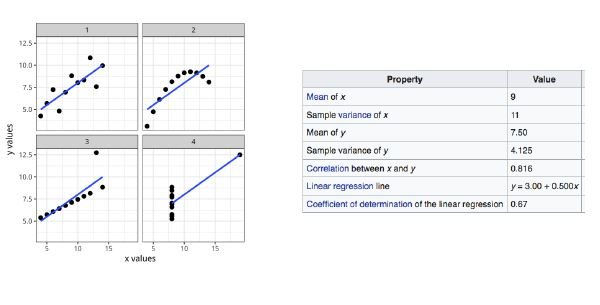
\includegraphics[width=\textwidth]{figures/MSDimage3}
\end{figure} the data has all of the same mean, sample variance, regression line, etc.

One important question that should be answered when presenting data visualizations is which type of plot is best. How do we know which type of graph is best for specific data as there are so many options(as seen in Figure 1), there are even more options how to specialise and spice up the data. Good plots are the goal, as they express the facts effectively as possible. Plots should be able to use encoding that people can easily decode, its has a clear and concise point. (see Mackinlay 1996 slide 9). Position of the plot, shape, size. color, line width, and even line type are very crucial when choosing the correct data visualization. The wrong visual will lead to improper interpretation, tread carefully reader. "Automating the Design of Graphical Presentations of Relational Information" b Jock University in 1986 was one of the first scientific paper that showed which visualizations are better than others. It showed that position in very influential, while color is not so much. It also went on to show that different strokes for different data types were and which were better. For example, Shape is not so influential for quantitative and ordinal data sets, but Shape is much more influential for nominal data sets. If the reader would like to learn more, a good book to read is "The Grammar of Graphics" by Springer or "ggplot2" by Hadley Wickham.
\subsection{R Studio: Working with ggplot}
During the last part of lecture, Professor Hofman quickly went over how to setup ggplot, and different types of plots and examples of such. First make sure you are running the Tidyverse, lubridate and scales libraries to start. Note that the ggplot histogram doesn't require a y, it associates the y as the count of the x function. Please, when you're reading this, open Professor Hofman's Github hub for visuals. We talked about how make bar charts, a normal histogram, a scatter plot histogram, line plots, and many more. While going through the examples keep in mind what is trying to be shown, and how each graph has its perks and drawbacks. We also go into to how to show question 3 on the homework, hint hint hint. And also how to label the charts, how to add color on the charts, and how to add error bars and confidence intervals. Please, Please go through the Github page, please it will be very beneficial



El Fin

   

%%% Local Variables:
%%% mode: latex
%%% TeX-master: t
%%% End:
